% ============================================================
%  BatchIt — Collaborative Bulk Purchasing Platform
%  SEN2241 · Group 13 · ICT University · Spring 2026
%  LaTeX Beamer Presentation — 10 Slides
% ============================================================
\documentclass[aspectratio=169,12pt]{beamer}

\usepackage[T1]{fontenc}
\usepackage[utf8]{inputenc}
\usepackage{helvet}
\renewcommand{\familydefault}{\sfdefault}
\usepackage{microtype}
\usepackage{xcolor}
\usepackage{tikz}
\usetikzlibrary{shapes.geometric,arrows.meta,positioning,calc,shadows,fit,backgrounds,decorations.pathreplacing}
\usepackage{pgfplots}
\pgfplotsset{compat=1.18}
\usepackage{booktabs}
\usepackage{colortbl}
\usepackage{tcolorbox}
\tcbuselibrary{skins,breakable,most}
\usepackage{listings}
\usepackage{adjustbox}
\usepackage{array}
\usepackage{tabularx}

% ── BatchIt Brand Palette ───────────────────────────────────
\definecolor{BITeal}    {HTML}{0B8A62}
\definecolor{BITealDk}  {HTML}{076B4B}
\definecolor{BITealLt}  {HTML}{1FB080}
\definecolor{BIOrange}  {HTML}{FFB347}
\definecolor{BIOrangeDk}{HTML}{E08A1A}
\definecolor{BICharcoal}{HTML}{1C2B24}
\definecolor{BISlate}   {HTML}{2E4A3E}
\definecolor{BILightBg} {HTML}{F0FAF5}
\definecolor{BIGray}    {HTML}{6B7C76}
\definecolor{BIWhite}   {HTML}{FFFFFF}
\definecolor{BICardBg}  {HTML}{E8F5EF}

% ── Custom Beamer Theme ─────────────────────────────────────
\usetheme{default}
\usecolortheme{default}
\setbeamertemplate{navigation symbols}{}

\setbeamercolor{background canvas}{bg=BIWhite}
\setbeamercolor{frametitle}{fg=BIWhite, bg=BITeal}
\setbeamerfont{frametitle}{series=\bfseries, size=\large}

\setbeamertemplate{frametitle}{%
  \begin{tikzpicture}[overlay, remember picture]
    \fill[BITeal] (current page.north west)
      rectangle ([yshift=-1.05cm]current page.north east);
    \node[anchor=west, text=BIWhite, font=\bfseries\large]
      at ([xshift=0.5cm, yshift=-0.52cm]current page.north west)
      {\insertframetitle};
    \fill[BIOrange] ([yshift=-1.05cm]current page.north west)
      rectangle ([yshift=-1.22cm, xshift=4cm]current page.north west);
  \end{tikzpicture}%
}

\setbeamertemplate{footline}{%
  \begin{tikzpicture}[overlay, remember picture]
    \fill[BICharcoal] (current page.south west)
      rectangle ([yshift=0.42cm]current page.south east);
    \node[anchor=west, text=BIGray, font=\tiny]
      at ([xshift=0.4cm, yshift=0.21cm]current page.south west)
      {BatchIt \textbullet{} SEN2241 \textbullet{} Group 13 \textbullet{} ICT University Spring 2026};
    \node[anchor=east, text=BIOrange, font=\small\bfseries]
      at ([xshift=-0.4cm, yshift=0.21cm]current page.south east)
      {\insertframenumber/\inserttotalframenumber};
  \end{tikzpicture}%
}

\setbeamercolor{block title}{fg=BIWhite, bg=BITeal}
\setbeamercolor{block body}{fg=BICharcoal, bg=BICardBg}
\setbeamerfont{block title}{series=\bfseries}
\setbeamercolor{item}{fg=BITeal}
\setbeamercolor{subitem}{fg=BIOrange}
\setbeamertemplate{itemize item}{\tikz\fill[BITeal](0,0)circle(2.2pt);}
\setbeamertemplate{itemize subitem}{\tikz\fill[BIOrange](0,0)--(4pt,0)--(2pt,3.5pt)--cycle;}

% ── tcolorbox styles ────────────────────────────────────────
\tcbset{
  cardbox/.style={enhanced,arc=5pt,boxrule=1pt,
    colframe=BITeal!40,colback=BICardBg,
    drop shadow={opacity=0.08},
    top=3pt,bottom=3pt,left=5pt,right=5pt,
    fonttitle=\bfseries\scriptsize,coltitle=BITeal},
  orangecard/.style={enhanced,arc=5pt,boxrule=1pt,
    colframe=BIOrange!60,colback=BIOrange!8,
    drop shadow={opacity=0.08},
    top=3pt,bottom=3pt,left=5pt,right=5pt,
    fonttitle=\bfseries\scriptsize,coltitle=BIOrangeDk},
  tealstat/.style={enhanced,arc=4pt,boxrule=0pt,
    colback=BITeal!12,colframe=BITeal,
    leftrule=4pt,rightrule=0pt,toprule=0pt,bottomrule=0pt,
    fonttitle=\bfseries\scriptsize,coltitle=BITeal,
    top=2pt,bottom=2pt,left=5pt,right=4pt},
  orangestat/.style={enhanced,arc=4pt,boxrule=0pt,
    colback=BIOrange!12,colframe=BIOrange,
    leftrule=4pt,rightrule=0pt,toprule=0pt,bottomrule=0pt,
    fonttitle=\bfseries\scriptsize,coltitle=BIOrangeDk,
    top=2pt,bottom=2pt,left=5pt,right=4pt},
  codebox/.style={enhanced,arc=5pt,boxrule=1pt,
    colframe=BITeal!50,colback=BICharcoal,
    top=3pt,bottom=3pt,left=5pt,right=5pt}
}

% ── listings ────────────────────────────────────────────────
\lstset{
  language=Python,
  basicstyle=\ttfamily\scriptsize\color{BITealLt},
  keywordstyle=\color{BIOrange}\bfseries,
  commentstyle=\color{BIGray},
  stringstyle=\color{BILightBg},
  backgroundcolor=\color{BICharcoal},
  frame=none,numbers=left,
  numberstyle=\tiny\color{BIGray},
  breaklines=true,tabsize=2,showstringspaces=false
}

% ── Arrow styles ────────────────────────────────────────────
\tikzset{
  myarr/.style={-{Stealth[length=5pt]},thick,color=BITeal},
  orrarr/.style={-{Stealth[length=5pt]},thick,color=BIOrange},
  dasharr/.style={-{Stealth[length=4pt]},dashed,color=BIGray,thin},
  inharr/.style={-{Triangle[open,length=6pt]},thick,color=BITeal},
  compar/.style={-{Diamond[open,length=6pt]},thick,color=BITealDk}
}

% ============================================================
\begin{document}
% ============================================================

%% SLIDE 1 — TITLE
{
\setbeamertemplate{footline}{}
\begin{frame}[plain]
\begin{tikzpicture}[overlay,remember picture]
  \fill[BICharcoal](current page.south west) rectangle (current page.north east);
  % Blobs
  \fill[BITeal,opacity=0.30]
    ([xshift=-2cm,yshift=-1.5cm]current page.north east) circle(4.8cm);
  \fill[BITealDk,opacity=0.35]
    ([xshift=2cm,yshift=1.5cm]current page.south west) circle(3.8cm);
  \fill[BIOrange,opacity=0.12]
    ([xshift=-1cm,yshift=0.8cm]current page.south east) circle(2.8cm);
  % Logo circle
  \fill[BITeal]   ($(current page.center)+(-4.6cm,1.2cm)$) circle(1.1cm);
  \draw[BIOrange,line width=3pt]
                  ($(current page.center)+(-4.6cm,1.2cm)$) circle(1.1cm);
  \node[font=\bfseries\LARGE,text=BIWhite]
    at ($(current page.center)+(-4.6cm,1.2cm)$) {B};
  % App name
  \node[anchor=west,font=\fontsize{34}{38}\selectfont\bfseries,text=BIWhite]
    at ($(current page.center)+(-3.1cm,1.25cm)$) {BatchIt};
  \node[anchor=west,font=\large\itshape,text=BIOrange]
    at ($(current page.center)+(-3.1cm,0.55cm)$) {Buy Together, Save Together};
  % Divider
  \fill[BITealLt]
    ($(current page.center)+(-3.1cm,-0.1cm)$)
    rectangle ($(current page.center)+(5.2cm,-0.25cm)$);
  % Subtitle
  \node[anchor=west,font=\normalsize,text=BILightBg]
    at ($(current page.center)+(-3.1cm,-0.65cm)$)
    {Mobile + REST API Application};
  \node[anchor=west,font=\small,text=BIGray]
    at ($(current page.center)+(-3.1cm,-1.1cm)$)
    {Flutter (Dart) \quad\textbullet\quad Django REST Framework \quad\textbullet\quad PostgreSQL \quad\textbullet\quad Jenkins CI/CD};
  % Tech tags
  \node[fill=BITeal,   text=BIWhite,font=\tiny\bfseries,rounded corners=3pt,inner xsep=5pt,inner ysep=2pt]
    at ($(current page.center)+(-2.2cm,-1.8cm)$) {FLUTTER};
  \node[fill=BIOrange, text=BIWhite,font=\tiny\bfseries,rounded corners=3pt,inner xsep=5pt,inner ysep=2pt]
    at ($(current page.center)+(-0.4cm,-1.8cm)$) {DJANGO};
  \node[fill=BITealLt, text=BIWhite,font=\tiny\bfseries,rounded corners=3pt,inner xsep=5pt,inner ysep=2pt]
    at ($(current page.center)+(1.5cm,-1.8cm)$) {POSTGRESQL};
  \node[fill=BISlate,  text=BIOrange,font=\tiny\bfseries,rounded corners=3pt,inner xsep=5pt,inner ysep=2pt]
    at ($(current page.center)+(3.5cm,-1.8cm)$) {JENKINS};
  % Course info
  \node[anchor=south west,font=\small,text=BIGray]
    at ([xshift=0.5cm,yshift=0.3cm]current page.south west)
    {Course: SEN2241 \quad Group 13 \quad Instructor: Tekoh Palma Achu \quad Spring 2026};
\end{tikzpicture}
\end{frame}
}

%% SLIDE 2 — INTRODUCTION & PROBLEM STATEMENT
\begin{frame}{Introduction \& Problem Statement}
\vspace{0.08cm}
\begin{columns}[T]
\begin{column}{0.54\textwidth}
  \begin{tcolorbox}[cardbox,title={What is BatchIt?}]
    \scriptsize A \textbf{mobile-first collaborative bulk purchasing} platform.
    Consumers form \emph{buying groups} (\textbf{batches}) to unlock
    wholesale prices on essential goods.
  \end{tcolorbox}
  \vspace{0.18cm}
  \begin{tcolorbox}[tealstat,title={Three Stakeholder Types}]
    \scriptsize
    \textbf{Customers} --- search \& join batches\\
    \textbf{Providers} --- verified businesses listing products\\
    \textbf{Admins} --- verify providers, ensure trust
  \end{tcolorbox}
  \vspace{0.18cm}
  \begin{tcolorbox}[orangestat,title={Inspired By}]
    \scriptsize
    Groupon (2008) model + Pinduoduo (2015) adapted for
    \textbf{mobile-first Sub-Saharan African commodity markets}.
  \end{tcolorbox}
\end{column}
\begin{column}{0.44\textwidth}
  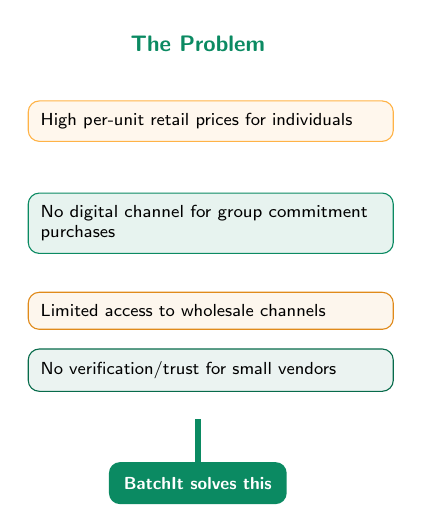
\begin{tikzpicture}[scale=0.9,transform shape]
    \node[font=\small\bfseries,text=BITeal] at (2.4,5.3) {The Problem};
    % Problem nodes — evenly spaced with 0.25cm gap between each
    \node[draw=BIOrange,fill=BIOrange!10,rounded corners=4pt,
          text width=4.8cm,font=\scriptsize,inner sep=5pt,anchor=north west]
      (p1) at (0,4.5) {High per-unit retail prices for individuals};
    \node[draw=BITeal,fill=BITeal!10,rounded corners=4pt,
          text width=4.8cm,font=\scriptsize,inner sep=5pt,anchor=north west]
      (p2) at (0,3.2) {No digital channel for group commitment purchases};
    \node[draw=BIOrangeDk,fill=BIOrangeDk!8,rounded corners=4pt,
          text width=4.8cm,font=\scriptsize,inner sep=5pt,anchor=north west]
      (p3) at (0,1.8) {Limited access to wholesale channels};
    \node[draw=BITealDk,fill=BITealDk!8,rounded corners=4pt,
          text width=4.8cm,font=\scriptsize,inner sep=5pt,anchor=north west]
      (p4) at (0,1.0) {No verification/trust for small vendors};
    % Arrow down
    \draw[myarr,line width=2pt] (2.4,0) -- (2.4,-0.8);
    % Solution box
    \node[fill=BITeal,text=BIWhite,font=\scriptsize\bfseries,
          rounded corners=4pt,inner sep=6pt] at (2.4,-0.9)
      {BatchIt solves this};
  \end{tikzpicture}
\end{column}
\end{columns}
\end{frame}

%% SLIDE 3 — SYSTEM ARCHITECTURE
\begin{frame}[fragile]{System Architecture}
\vspace{-0.1cm}
\begin{center}
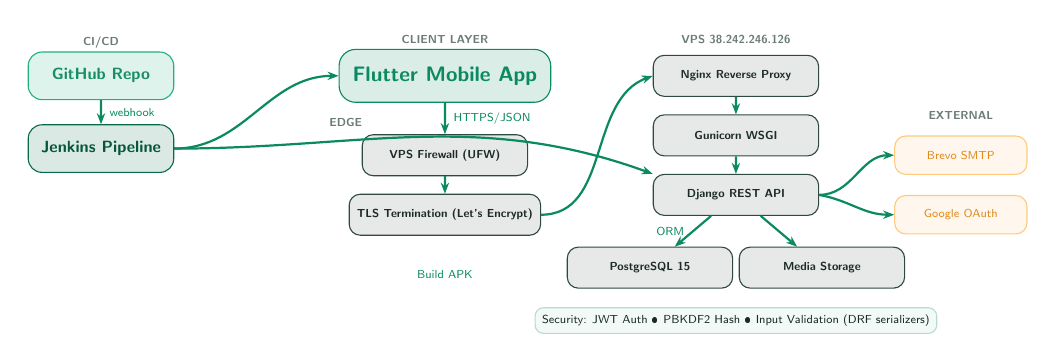
\begin{tikzpicture}[scale=0.84,transform shape,
  layer/.style={draw=#1,fill=#1!15,rounded corners=5pt,
                minimum width=2.8cm,minimum height=0.72cm,
                font=\scriptsize\bfseries,text=#1!80!black},
  srv/.style={draw=BISlate,fill=BISlate!12,rounded corners=4pt,
              minimum width=2.5cm,minimum height=0.62cm,
              font=\tiny\bfseries,text=BICharcoal},
  ext/.style={draw=BIOrange!70,fill=BIOrange!10,rounded corners=4pt,
              minimum width=2cm,minimum height=0.58cm,
              font=\tiny,text=BIOrangeDk},
  lbl/.style={font=\tiny\bfseries,text=BIGray},
  arr/.style={-{Stealth[length=4pt]},thick,BITeal}
]
  % CI/CD
  \node[layer=BITealLt,minimum width=2.2cm] (gh)  at (-5.2, 3.2) {GitHub Repo};
  \node[layer=BITealDk,minimum width=2.2cm] (jk)  at (-5.2, 2.1) {Jenkins Pipeline};
  \node[lbl] at (-5.2,3.7) {CI/CD};

  % Client
  \node[draw=BITeal,fill=BITeal!15,rounded corners=6pt,
        minimum width=3.2cm,minimum height=0.8cm,
        font=\small\bfseries,text=BITeal] (fl) at (0,3.2) {Flutter Mobile App};
  \node[lbl] at (0,3.75) {CLIENT LAYER};

  % Edge
  \node[srv] (fw)  at (0,2.0) {VPS Firewall (UFW)};
  \node[srv] (tls) at (0,1.1) {TLS Termination (Let's Encrypt)};
  \node[lbl] at (-1.5,2.5) {EDGE};

  % VPS stack
  \node[lbl] at (4.4,3.75) {VPS 38.242.246.126};
  \node[srv]  (ng) at (4.4,3.2) {Nginx Reverse Proxy};
  \node[srv]  (gu) at (4.4,2.3) {Gunicorn WSGI};
  \node[srv]  (dj) at (4.4,1.4) {Django REST API};
  \node[srv]  (pg) at (3.1,0.3) {PostgreSQL 15};
  \node[srv]  (ms) at (5.7,0.3) {Media Storage};

  % External
  \node[lbl]  at (7.8,2.6) {EXTERNAL};
  \node[ext]  (br) at (7.8,2.0) {Brevo SMTP};
  \node[ext]  (go) at (7.8,1.1) {Google OAuth};

  % Arrows
  \draw[arr] (gh) -- (jk) node[midway,right,font=\tiny]{webhook};
  \draw[arr] (jk.east) to[out=0,in=180] (fl.west)
    node[near end,above,font=\tiny]{Build APK};
  \draw[arr] (jk.east) to[out=0,in=160] (dj.north west);
  \draw[arr] (fl)  -- (fw)  node[midway,right,font=\tiny]{HTTPS/JSON};
  \draw[arr] (fw)  -- (tls);
  \draw[arr] (tls.east) to[out=0,in=200] (ng.west);
  \draw[arr] (ng)  -- (gu);
  \draw[arr] (gu)  -- (dj);
  \draw[arr] (dj)  -- (pg) node[midway,left,font=\tiny]{ORM};
  \draw[arr] (dj)  -- (ms);
  \draw[arr] (dj.east) to[out=0,in=180]  (br.west);
  \draw[arr] (dj.east) to[out=-10,in=180](go.west);

  % Security controls legend
  \node[draw=BITeal!30,fill=BITeal!5,rounded corners=3pt,
        font=\tiny,text=BICharcoal,inner sep=3pt] at (4.4,-0.5)
    {Security: JWT Auth \textbullet{} PBKDF2 Hash \textbullet{} Input Validation (DRF serializers)};
\end{tikzpicture}
\end{center}
\end{frame}

%% SLIDE 4 — KEY FEATURES
\begin{frame}{Key Features}
\vspace{0.08cm}
\begin{columns}[T]
\begin{column}{0.49\textwidth}
  \begin{tcolorbox}[cardbox,title={Batch Lifecycle Management}]
    \scriptsize Create \(\to\) Discover \(\to\) Join \(\to\) Fill \(\to\) Complete.
    Live \textbf{progress bar}. Auto status transitions (open/filled/expired).
  \end{tcolorbox}\vspace{0.14cm}
  \begin{tcolorbox}[cardbox,title={Dual Authentication}]
    \scriptsize Email/password + \textbf{6-digit code} via Brevo SMTP, plus
    \textbf{Google OAuth 2.0}. JWT: 60 min access, 7 day refresh.
  \end{tcolorbox}\vspace{0.14cm}
  \begin{tcolorbox}[cardbox,title={Provider Verification Workflow}]
    \scriptsize Business submits docs $\to$ Admin reviews $\to$ Approved/Rejected
    with in-app notification.
  \end{tcolorbox}\vspace{0.14cm}
  \begin{tcolorbox}[cardbox,title={Bilingual UI (EN / FR) + Themes}]
    \scriptsize Full Material Design 3 with light/dark toggle.
    French localization persists across restarts.
  \end{tcolorbox}
\end{column}
\begin{column}{0.49\textwidth}
  \begin{tcolorbox}[orangecard,title={Batch Group Chat}]
    \scriptsize Each batch has a \textbf{persistent group chat room}.
    REST polling (POST messages / GET history). Coordinate with buyers.
  \end{tcolorbox}\vspace{0.14cm}
  \begin{tcolorbox}[orangecard,title={Map-Based Discovery}]
    \scriptsize OpenStreetMap via \texttt{flutter\_map}. View providers and
    batches by \textbf{geographic proximity}. Tap pins for detail.
  \end{tcolorbox}\vspace{0.14cm}
  \begin{tcolorbox}[orangecard,title={In-App Notifications}]
    \scriptsize Triggered on batch creation, join, fill, and provider approval.
    Unread badge count. Provider subscription model.
  \end{tcolorbox}\vspace{0.14cm}
  \begin{tcolorbox}[orangecard,title={Orders, Profile \& 40+ REST Endpoints}]
    \scriptsize Full order history, profile photo upload.
    Swagger/OpenAPI docs via \texttt{drf-yasg}.
  \end{tcolorbox}
\end{column}
\end{columns}
\end{frame}

%% SLIDE 5 — CLASS DIAGRAM
\begin{frame}{Object-Oriented Design --- Core Class Diagram}
\vspace{-0.05cm}
\begin{center}
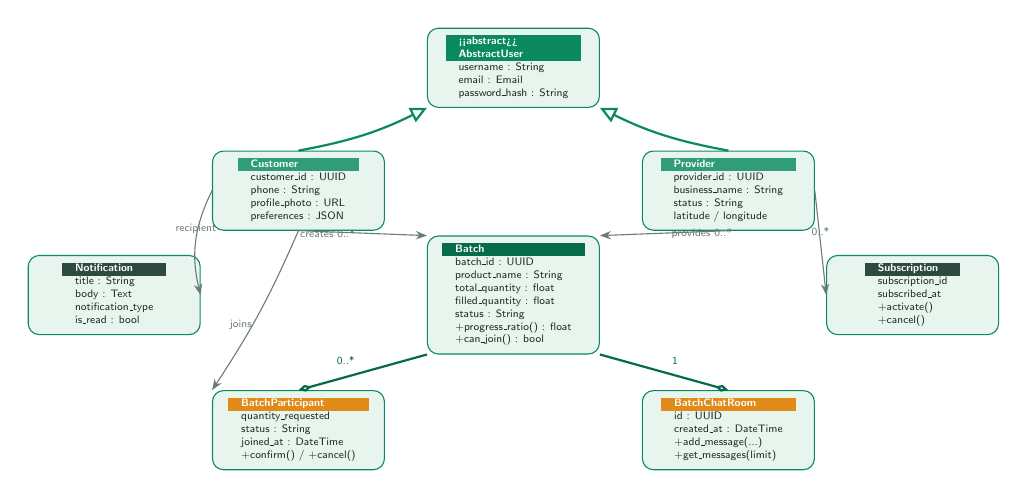
\begin{tikzpicture}[scale=0.78,transform shape,
  cls/.style={draw=BITeal,fill=BICardBg,rounded corners=4pt,
              minimum width=2.8cm,font=\tiny,text=BICharcoal},
  fk/.style={-{Stealth[length=4pt]},BIGray,thin},
  inh/.style={-{Triangle[open,length=6pt]},thick,BITeal},
  cmp/.style={-{Diamond[open,length=5pt]},thick,BITealDk}
]
% AbstractUser
\node[cls] (au) at (0,4.6) {%
  \begin{tabular}{l}
    \rowcolor{BITeal}\color{BIWhite}\textbf{<<abstract>>}\\
    \rowcolor{BITeal}\color{BIWhite}\textbf{AbstractUser}\\
    username : String\\
    email : Email\\
    password\_hash : String
  \end{tabular}};

% Customer
\node[cls] (cu) at (-3.5,2.6) {%
  \begin{tabular}{l}
    \rowcolor{BITeal!85}\color{BIWhite}\textbf{Customer}\\
    customer\_id : UUID\\
    phone : String\\
    profile\_photo : URL\\
    preferences : JSON
  \end{tabular}};

% Provider
\node[cls] (pv) at (3.5,2.6) {%
  \begin{tabular}{l}
    \rowcolor{BITeal!85}\color{BIWhite}\textbf{Provider}\\
    provider\_id : UUID\\
    business\_name : String\\
    status : String\\
    latitude / longitude
  \end{tabular}};

% Batch
\node[cls] (ba) at (0,0.9) {%
  \begin{tabular}{l}
    \rowcolor{BITealDk}\color{BIWhite}\textbf{Batch}\\
    batch\_id : UUID\\
    product\_name : String\\
    total\_quantity : float\\
    filled\_quantity : float\\
    status : String\\
    +progress\_ratio() : float\\
    +can\_join() : bool
  \end{tabular}};

% BatchParticipant
\node[cls] (bp) at (-3.5,-1.3) {%
  \begin{tabular}{l}
    \rowcolor{BIOrangeDk}\color{BIWhite}\textbf{BatchParticipant}\\
    quantity\_requested\\
    status : String\\
    joined\_at : DateTime\\
    +confirm() / +cancel()
  \end{tabular}};

% BatchChatRoom
\node[cls] (bc) at (3.5,-1.3) {%
  \begin{tabular}{l}
    \rowcolor{BIOrangeDk}\color{BIWhite}\textbf{BatchChatRoom}\\
    id : UUID\\
    created\_at : DateTime\\
    +add\_message(...)\\
    +get\_messages(limit)
  \end{tabular}};

% Notification
\node[cls] (no) at (-6.5,0.9) {%
  \begin{tabular}{l}
    \rowcolor{BISlate}\color{BIWhite}\textbf{Notification}\\
    title : String\\
    body : Text\\
    notification\_type\\
    is\_read : bool
  \end{tabular}};

% Subscription
\node[cls] (sb) at (6.5,0.9) {%
  \begin{tabular}{l}
    \rowcolor{BISlate}\color{BIWhite}\textbf{Subscription}\\
    subscription\_id\\
    subscribed\_at\\
    +activate()\\
    +cancel()
  \end{tabular}};

% Relationships
\draw[inh] (cu.north) to[bend right=8] (au.south west);
\draw[inh] (pv.north) to[bend left=8]  (au.south east);
\draw[fk]  (cu.south) to node[left,font=\tiny]{creates 0..*}    (ba.north west);
\draw[fk]  (pv.south) to node[right,font=\tiny]{provides 0..*} (ba.north east);
\draw[cmp] (ba.south west) to node[above left,font=\tiny]{0..*} (bp.north);
\draw[cmp] (ba.south east) to node[above right,font=\tiny]{1}   (bc.north);
\draw[fk]  (cu.west) to[bend right=20] node[above,font=\tiny]{recipient}(no.east);
\draw[fk]  (cu.south) to[bend left=5]  node[below left,font=\tiny]{joins}(bp.north west);
\draw[fk]  (pv.east) to node[above,font=\tiny]{0..*}(sb.west);
\end{tikzpicture}
\end{center}
\end{frame}

%% SLIDE 6 — SEQUENCE DIAGRAMS
\begin{frame}{Critical Sequence Flows}
\vspace{0.06cm}
\begin{columns}[T]
\begin{column}{0.49\textwidth}
  {\small\bfseries\color{BITeal} SD1 --- Email Registration + Verification}
  \vspace{0.1cm}

  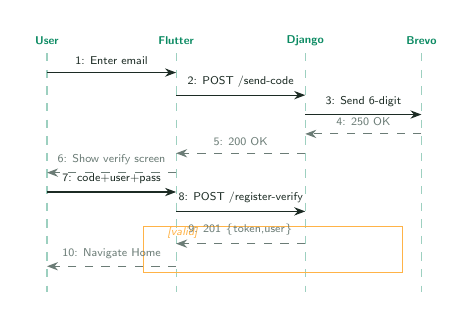
\begin{tikzpicture}[scale=0.82,transform shape,
    life/.style={draw=BITeal!40,dashed,thin},
    fwd/.style={-{Stealth[length=4pt]},BICharcoal,thin},
    bck/.style={-{Stealth[length=4pt]},BIGray,dashed,thin},
    hd/.style={font=\tiny\bfseries,text=BITeal,align=center}
  ]
    \node[hd](U) at (0,3.7)    {User};
    \node[hd](A) at (2.0,3.7)  {Flutter};
    \node[hd](D) at (4.0,3.7)  {Django};
    \node[hd](E) at (5.8,3.7)  {Brevo};
    \foreach \x in {0,2.0,4.0,5.8}
      \draw[life](\x,3.5)--(\x,-0.2);
    \draw[fwd](0,3.2)--node[above,font=\tiny]{1: Enter email}(2.0,3.2);
    \draw[fwd](2.0,2.85)--node[above,font=\tiny]{2: POST /send-code}(4.0,2.85);
    \draw[fwd](4.0,2.55)--node[above,font=\tiny]{3: Send 6-digit}(5.8,2.55);
    \draw[bck](5.8,2.25)--node[above,font=\tiny]{4: 250 OK}(4.0,2.25);
    \draw[bck](4.0,1.95)--node[above,font=\tiny]{5: 200 OK}(2.0,1.95);
    \draw[bck](2.0,1.65)--node[above,font=\tiny]{6: Show verify screen}(0,1.65);
    \draw[fwd](0,1.35)--node[above,font=\tiny]{7: code+user+pass}(2.0,1.35);
    \draw[fwd](2.0,1.05)--node[above,font=\tiny]{8: POST /register-verify}(4.0,1.05);
    \draw[BIOrange,thin](1.5,0.82) rectangle (5.5,0.1);
    \node[font=\tiny\itshape,text=BIOrange] at (2.1,0.72){[valid]};
    \draw[bck](4.0,0.55)--node[above,font=\tiny]{9: 201 \{token,user\}}(2.0,0.55);
    \draw[bck](2.0,0.2)--node[above,font=\tiny]{10: Navigate Home}(0,0.2);
  \end{tikzpicture}
\end{column}
\begin{column}{0.49\textwidth}
  {\small\bfseries\color{BITeal} SD4 --- Customer Joins a Batch}
  \vspace{0.1cm}

  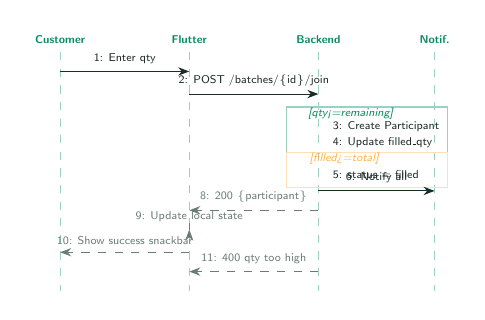
\begin{tikzpicture}[scale=0.82,transform shape,
    life/.style={draw=BITeal!40,dashed,thin},
    fwd/.style={-{Stealth[length=4pt]},BICharcoal,thin},
    bck/.style={-{Stealth[length=4pt]},BIGray,dashed,thin},
    hd/.style={font=\tiny\bfseries,text=BITeal,align=center}
  ]
    \node[hd](C) at (0,3.7)   {Customer};
    \node[hd](F) at (2.0,3.7) {Flutter};
    \node[hd](B) at (4.0,3.7) {Backend};
    \node[hd](N) at (5.8,3.7) {Notif.};
    \foreach \x in {0,2.0,4.0,5.8}
      \draw[life](\x,3.5)--(\x,-0.2);
    \draw[fwd](0,3.2)--node[above,font=\tiny]{1: Enter qty}(2.0,3.2);
    \draw[fwd](2.0,2.85)--node[above,font=\tiny]{2: POST /batches/\{id\}/join}(4.0,2.85);
    \draw[BITeal!40,thin](3.5,2.65) rectangle (6.0,1.4);
    \node[font=\tiny\itshape,text=BITeal] at (4.5,2.55){[qty<=remaining]};
    \node[font=\tiny,text=BICharcoal,anchor=west] at (4.1,2.35){3: Create Participant};
    \node[font=\tiny,text=BICharcoal,anchor=west] at (4.1,2.1) {4: Update filled\_qty};
    \draw[BIOrange!40,thin](3.5,1.95) rectangle (6.0,1.4);
    \node[font=\tiny\itshape,text=BIOrange] at (4.4,1.85){[filled>=total]};
    \node[font=\tiny,text=BICharcoal,anchor=west] at (4.1,1.6){5: status = filled};
    \draw[fwd](4.0,1.35)--node[above,font=\tiny]{6: Notify all}(5.8,1.35);
    \draw[bck](4.0,1.05)--node[above,font=\tiny]{8: 200 \{participant\}}(2.0,1.05);
    \draw[bck](2.0,0.75)--node[above,font=\tiny]{9: Update local state}(2.0,0.75);
    \draw[bck](2.0,0.4)--node[above,font=\tiny]{10: Show success snackbar}(0,0.4);
    \draw[bck](4.0,0.1)--node[above,font=\tiny]{11: 400 qty too high}(2.0,0.1);
  \end{tikzpicture}
\end{column}
\end{columns}
\end{frame}

%% SLIDE 7 — SCRUM & TEAM
\begin{frame}{Scrum Methodology \& Team Organisation}
\vspace{0.06cm}
\begin{columns}[T]
\begin{column}{0.53\textwidth}
  {\small\bfseries\color{BITeal} 4 Sprints \textbullet{} GitHub Projects Kanban \textbullet{} Feature Branches}
  \vspace{0.15cm}

  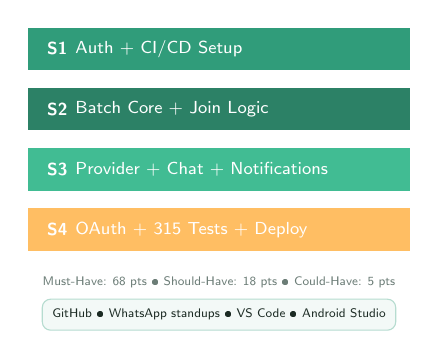
\begin{tikzpicture}[scale=0.9,transform shape]
    % Sprint bars
    \fill[BITeal!85]    (0,3.6) rectangle (5.4,4.2);
    \fill[BITealDk!85]  (0,2.75) rectangle (5.4,3.35);
    \fill[BITealLt!85]  (0,1.9) rectangle (5.4,2.5);
    \fill[BIOrange!85]  (0,1.05) rectangle (5.4,1.65);
    % Sprint labels
    \node[anchor=west,font=\scriptsize\bfseries,text=BIWhite] at (0.15,3.9) {S1};
    \node[anchor=west,font=\scriptsize,text=BIWhite]          at (0.55,3.9) {Auth + CI/CD Setup};
    \node[anchor=west,font=\scriptsize\bfseries,text=BIWhite] at (0.15,3.05){S2};
    \node[anchor=west,font=\scriptsize,text=BIWhite]          at (0.55,3.05){Batch Core + Join Logic};
    \node[anchor=west,font=\scriptsize\bfseries,text=BIWhite] at (0.15,2.2) {S3};
    \node[anchor=west,font=\scriptsize,text=BIWhite]          at (0.55,2.2) {Provider + Chat + Notifications};
    \node[anchor=west,font=\scriptsize\bfseries,text=BIWhite] at (0.15,1.35){S4};
    \node[anchor=west,font=\scriptsize,text=BIWhite]          at (0.55,1.35){OAuth + 315 Tests + Deploy};
    % Story points note
    \node[font=\tiny,text=BIGray] at (2.7,0.6)
      {Must-Have: 68 pts \textbullet{} Should-Have: 18 pts \textbullet{} Could-Have: 5 pts};
    % Methodology note
    \node[draw=BITeal!30,fill=BITeal!5,rounded corners=3pt,
          font=\tiny,text=BICharcoal,inner sep=4pt] at (2.7,0.15)
      {GitHub \textbullet{} WhatsApp standups \textbullet{} VS Code \textbullet{} Android Studio};
  \end{tikzpicture}
\end{column}
\begin{column}{0.44\textwidth}
  {\small\bfseries\color{BITeal} Team Roles (5 Members)}
  \vspace{0.15cm}

  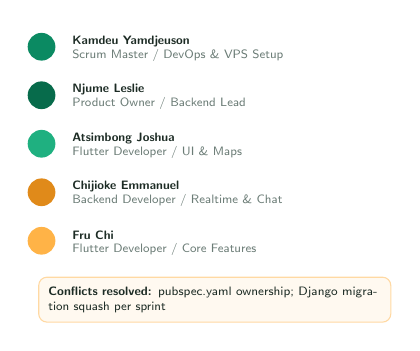
\begin{tikzpicture}[scale=0.88,transform shape]
    % Member 1
    \fill[BITeal]     (0,4.0) circle(0.2cm);
    \node[font=\tiny\bfseries,text=BICharcoal,anchor=west] at (0.32,4.08) {Kamdeu Yamdjeuson};
    \node[font=\tiny,text=BIGray,anchor=west]              at (0.32,3.88) {Scrum Master / DevOps \& VPS Setup};
    % Member 2
    \fill[BITealDk]   (0,3.3) circle(0.2cm);
    \node[font=\tiny\bfseries,text=BICharcoal,anchor=west] at (0.32,3.38) {Njume Leslie};
    \node[font=\tiny,text=BIGray,anchor=west]              at (0.32,3.18) {Product Owner / Backend Lead};
    % Member 3
    \fill[BITealLt]   (0,2.6) circle(0.2cm);
    \node[font=\tiny\bfseries,text=BICharcoal,anchor=west] at (0.32,2.68) {Atsimbong Joshua};
    \node[font=\tiny,text=BIGray,anchor=west]              at (0.32,2.48) {Flutter Developer / UI \& Maps};
    % Member 4
    \fill[BIOrangeDk] (0,1.9) circle(0.2cm);
    \node[font=\tiny\bfseries,text=BICharcoal,anchor=west] at (0.32,1.98) {Chijioke Emmanuel};
    \node[font=\tiny,text=BIGray,anchor=west]              at (0.32,1.78) {Backend Developer / Realtime \& Chat};
    % Member 5
    \fill[BIOrange]   (0,1.2) circle(0.2cm);
    \node[font=\tiny\bfseries,text=BICharcoal,anchor=west] at (0.32,1.28) {Fru Chi};
    \node[font=\tiny,text=BIGray,anchor=west]              at (0.32,1.08) {Flutter Developer / Core Features};
    % Conflict resolution
    \node[draw=BIOrange!50,fill=BIOrange!8,rounded corners=3pt,
          font=\tiny,text=BICharcoal,inner sep=4pt,text width=4.8cm] at (2.5,0.35)
      {\textbf{Conflicts resolved:} pubspec.yaml ownership; Django migration squash per sprint};
  \end{tikzpicture}
\end{column}
\end{columns}
\end{frame}

%% SLIDE 8 — ALGORITHMS & API
\begin{frame}[fragile]{Core Algorithms \& API Design}
\vspace{0.05cm}
\begin{columns}[T]
\begin{column}{0.56\textwidth}
  {\small\bfseries\color{BITeal} Batch Fill Algorithm (Django views.py)}
  \vspace{0.08cm}

  \begin{tcolorbox}[codebox]
\begin{lstlisting}
def join_batch(request, batch_id):
    batch = Batch.objects.get(batch_id=batch_id)
    qty = request.data['quantity_requested']

    # Guard: batch must be open
    if batch.status != 'open':
        raise ValidationError("Batch is not open.")

    # Guard: quantity check
    remaining = (batch.total_quantity
                 - batch.filled_quantity)
    if qty > remaining:
        raise ValidationError(
            f"Only {remaining} units left.")

    # Create participant + atomic update
    BatchParticipant.objects.create(
        batch=batch, customer=request.user,
        quantity_requested=qty, status='pending')

    batch.filled_quantity += qty
    if batch.filled_quantity >= batch.total_quantity:
        batch.status = 'filled'
        notify_all_participants(batch, "Batch full!")
    batch.save()
    return Response(ParticipantSerializer(...).data)
\end{lstlisting}
  \end{tcolorbox}
\end{column}
\begin{column}{0.42\textwidth}
  {\small\bfseries\color{BITeal} Selected REST Endpoints}
  \vspace{0.1cm}

  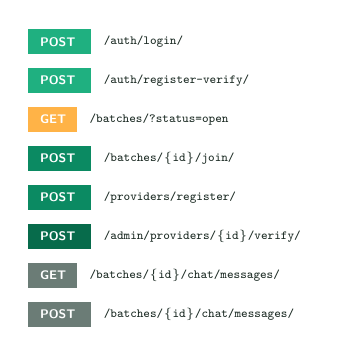
\begin{tikzpicture}[scale=0.9,transform shape]
    % POST
    \fill[BITealLt]   (0,5.5) rectangle (0.9,5.85);
    \node[font=\tiny\bfseries,text=BIWhite,anchor=west] at (0.05,5.67) {POST};
    \node[font=\tiny\ttfamily,text=BICharcoal,anchor=west] at (0.95,5.67) {/auth/login/};

    \fill[BITealLt]   (0,4.95) rectangle (0.9,5.3);
    \node[font=\tiny\bfseries,text=BIWhite,anchor=west] at (0.05,5.12) {POST};
    \node[font=\tiny\ttfamily,text=BICharcoal,anchor=west] at (0.95,5.12) {/auth/register-verify/};

    \fill[BIOrange]   (0,4.4) rectangle (0.7,4.75);
    \node[font=\tiny\bfseries,text=BIWhite,anchor=west] at (0.05,4.57) {GET};
    \node[font=\tiny\ttfamily,text=BICharcoal,anchor=west] at (0.75,4.57) {/batches/?status=open};

    \fill[BITeal]     (0,3.85) rectangle (0.9,4.2);
    \node[font=\tiny\bfseries,text=BIWhite,anchor=west] at (0.05,4.02) {POST};
    \node[font=\tiny\ttfamily,text=BICharcoal,anchor=west] at (0.95,4.02) {/batches/\{id\}/join/};

    \fill[BITeal]     (0,3.3) rectangle (0.9,3.65);
    \node[font=\tiny\bfseries,text=BIWhite,anchor=west] at (0.05,3.47) {POST};
    \node[font=\tiny\ttfamily,text=BICharcoal,anchor=west] at (0.95,3.47) {/providers/register/};

    \fill[BITealDk]   (0,2.75) rectangle (0.9,3.1);
    \node[font=\tiny\bfseries,text=BIWhite,anchor=west] at (0.05,2.92) {POST};
    \node[font=\tiny\ttfamily,text=BICharcoal,anchor=west] at (0.95,2.92) {/admin/providers/\{id\}/verify/};

    \fill[BIGray]     (0,2.2) rectangle (0.7,2.55);
    \node[font=\tiny\bfseries,text=BIWhite,anchor=west] at (0.05,2.37) {GET};
    \node[font=\tiny\ttfamily,text=BICharcoal,anchor=west] at (0.75,2.37) {/batches/\{id\}/chat/messages/};

    \fill[BIGray]     (0,1.65) rectangle (0.9,2.0);
    \node[font=\tiny\bfseries,text=BIWhite,anchor=west] at (0.05,1.82) {POST};
    \node[font=\tiny\ttfamily,text=BICharcoal,anchor=west] at (0.95,1.82) {/batches/\{id\}/chat/messages/};
  \end{tikzpicture}

  \vspace{0.12cm}
  \begin{tcolorbox}[tealstat,title={API Stats}]
    \scriptsize \textbf{40+} endpoints \textbullet{} JWT Auth\\
    Swagger/OpenAPI via \texttt{drf-yasg}\\
    PBKDF2 password hashing
  \end{tcolorbox}
\end{column}
\end{columns}
\end{frame}

%% SLIDE 9 — CI/CD + TEST COVERAGE
\begin{frame}[fragile]{CI/CD Pipeline \& Test Coverage}
\vspace{0.05cm}
\begin{columns}[T]
\begin{column}{0.49\textwidth}
  {\small\bfseries\color{BITeal} Jenkins Pipeline --- Triggered on Every Push to \texttt{main}}
  \vspace{0.15cm}

  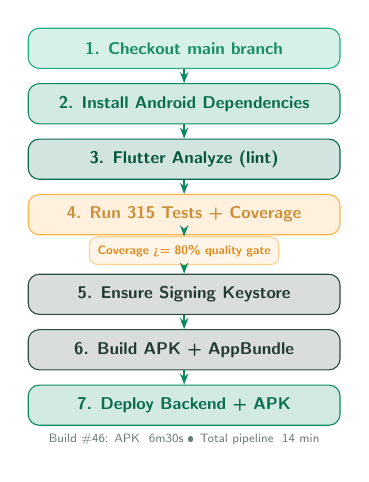
\begin{tikzpicture}[scale=0.88,transform shape,
    stg/.style={draw=#1,fill=#1!18,rounded corners=4pt,
                minimum width=4.5cm,minimum height=0.58cm,
                font=\scriptsize\bfseries,text=#1!80!black},
    ar/.style={-{Stealth[length=4pt]},thick,BITeal}
  ]
    \node[stg=BITealLt]  (s1) at (0,4.0) {1. Checkout main branch};
    \node[stg=BITeal]    (s2) at (0,3.2) {2. Install Android Dependencies};
    \node[stg=BITealDk]  (s3) at (0,2.4) {3. Flutter Analyze (lint)};
    \node[stg=BIOrange]  (s4) at (0,1.6) {4. Run 315 Tests + Coverage};
    \node[draw=BIOrange!60,fill=BIOrange!12,rounded corners=3pt,
          font=\tiny\bfseries,text=BIOrangeDk,
          minimum width=2.5cm,minimum height=0.38cm] (gate) at (0,1.08)
         {Coverage >= 80\% quality gate};
    \node[stg=BISlate]   (s5) at (0,0.45) {5. Ensure Signing Keystore};
    \node[stg=BISlate]   (s6) at (0,-0.35){6. Build APK + AppBundle};
    \node[stg=BITeal]    (s7) at (0,-1.15){7. Deploy Backend + APK};
    \foreach \a/\b in {s1/s2,s2/s3,s3/s4,s4/gate,gate/s5,s5/s6,s6/s7}
      \draw[ar](\a.south)--(\b.north);
    \node[font=\tiny,text=BIGray] at (0,-1.65)
      {Build \#46: APK ~6m30s \textbullet{} Total pipeline ~14 min};
  \end{tikzpicture}
\end{column}
\begin{column}{0.49\textwidth}
  {\small\bfseries\color{BITeal} Test Coverage --- Build \#46 (83.6\% overall)}
  \vspace{0.1cm}

  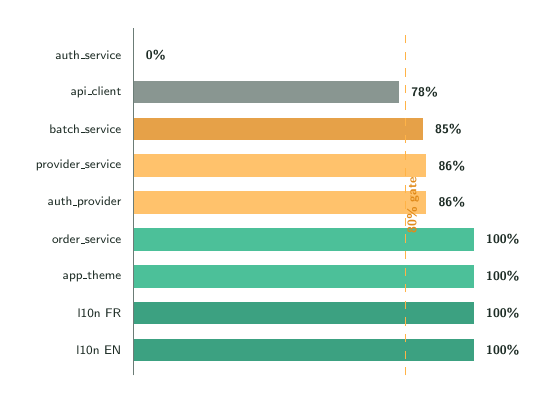
\begin{tikzpicture}[scale=0.9,transform shape]
    % Bar chart manual
    \foreach \i/\pct/\lbl/\col in {
      1/100/l10n EN/BITeal,
      2/100/l10n FR/BITeal,
      3/100/app\_theme/BITealLt,
      4/100/order\_service/BITealLt,
      5/86/auth\_provider/BIOrange,
      6/86/provider\_service/BIOrange,
      7/85/batch\_service/BIOrangeDk,
      8/78/api\_client/BIGray,
      9/0/auth\_service/BICharcoal%
    }{
      \pgfmathsetmacro{\barw}{\pct*0.048}
      \colorlet{barcol}{\col!80}%
      \fill[barcol](0,\i*0.52-0.42) rectangle (\barw,\i*0.52-0.1);
      \node[font=\tiny,text=BICharcoal,anchor=east] at (-0.05,\i*0.52-0.26) {\lbl};
      \node[font=\tiny\bfseries,text=BICharcoal,anchor=west] at (\barw+0.05,\i*0.52-0.26) {\pct\%};
    }
    \draw[BIGray,thin](0,-0.1)--(0,4.8);
    % 80% gate line
    \pgfmathsetmacro{\gatex}{80*0.048}
    \draw[BIOrange,dashed,thin](\gatex,-0.1)--(\gatex,4.8);
    \node[font=\tiny\bfseries,text=BIOrangeDk,rotate=90] at (\gatex+0.1,2.3){80\% gate};
  \end{tikzpicture}

  \vspace{0.1cm}
  \begin{tcolorbox}[tealstat,title={Test Suite Stats}]
    \scriptsize
    \textbf{315 tests} --- all passing\\
    \textbf{83.6\%} line coverage (1466 / 1753 lines)\\
    Packages: \texttt{mocktail} + \texttt{flutter\_test}\\
    Started at 28.3\% --- improved systematically
  \end{tcolorbox}
\end{column}
\end{columns}
\end{frame}

%% SLIDE 10 — RESULTS & CONCLUSION
\begin{frame}{Results, Future Work \& Conclusion}
\vspace{0.05cm}
\begin{columns}[T]
\begin{column}{0.48\textwidth}
  {\small\bfseries\color{BITeal} Achievements}
  \vspace{0.1cm}

  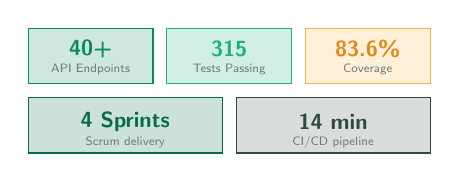
\begin{tikzpicture}[scale=0.88,transform shape]
    % Stat boxes
    \fill[BITeal!20]    (0,2.8)  rectangle (1.8,3.6);
    \draw[BITeal,thin]  (0,2.8)  rectangle (1.8,3.6);
    \node[font=\small\bfseries,text=BITeal]     at (0.9,3.3)  {40+};
    \node[font=\tiny,text=BIGray,align=center]  at (0.9,3.0)  {API Endpoints};

    \fill[BITealLt!20]  (2.0,2.8) rectangle (3.8,3.6);
    \draw[BITealLt,thin](2.0,2.8) rectangle (3.8,3.6);
    \node[font=\small\bfseries,text=BITealLt]   at (2.9,3.3)  {315};
    \node[font=\tiny,text=BIGray,align=center]  at (2.9,3.0)  {Tests Passing};

    \fill[BIOrange!20]  (4.0,2.8) rectangle (5.8,3.6);
    \draw[BIOrange,thin](4.0,2.8) rectangle (5.8,3.6);
    \node[font=\small\bfseries,text=BIOrangeDk] at (4.9,3.3)  {83.6\%};
    \node[font=\tiny,text=BIGray,align=center]  at (4.9,3.0)  {Coverage};

    \fill[BITealDk!20]  (0,1.8)   rectangle (2.8,2.6);
    \draw[BITealDk,thin](0,1.8)   rectangle (2.8,2.6);
    \node[font=\small\bfseries,text=BITealDk]   at (1.4,2.25) {4 Sprints};
    \node[font=\tiny,text=BIGray,align=center]  at (1.4,1.95) {Scrum delivery};

    \fill[BISlate!18]   (3.0,1.8) rectangle (5.8,2.6);
    \draw[BISlate,thin] (3.0,1.8) rectangle (5.8,2.6);
    \node[font=\small\bfseries,text=BISlate]    at (4.4,2.25) {14 min};
    \node[font=\tiny,text=BIGray,align=center]  at (4.4,1.95) {CI/CD pipeline};
  \end{tikzpicture}

  \vspace{0.18cm}
  \begin{tcolorbox}[cardbox]
    \scriptsize
    \begin{itemize}\setlength\itemsep{1pt}
      \item Full-stack Flutter + Django in 4 weeks
      \item Bilingual EN/FR Material Design 3 UI
      \item Production VPS: \texttt{batchit.duckdns.org}
      \item Signed APK auto-built via Jenkins
      \item 40+ documented REST API endpoints
    \end{itemize}
  \end{tcolorbox}

  \vspace{0.12cm}
  \begin{tcolorbox}[orangestat,title={Challenges Overcome}]
    \scriptsize Jenkins keystore path \textbullet{} Google SHA-1 mismatch\\
    Coverage 28\% $\to$ 83.6\% \textbullet{} JWT migration
  \end{tcolorbox}
\end{column}
\begin{column}{0.5\textwidth}
  {\small\bfseries\color{BITeal} Recommendations for Future Work}
  \vspace{0.12cm}

  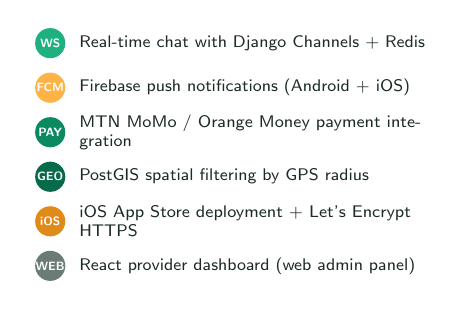
\begin{tikzpicture}[scale=0.87,transform shape]
    % Future items
    \fill[BITealLt]   (0,5.3) circle(0.22cm);
    \node[font=\tiny\bfseries,text=BIWhite] at (0,5.3){WS};
    \node[font=\scriptsize,text=BICharcoal,anchor=west,text width=5.1cm]
      at (0.3,5.3){Real-time chat with Django Channels + Redis};

    \fill[BIOrange]   (0,4.65) circle(0.22cm);
    \node[font=\tiny\bfseries,text=BIWhite] at (0,4.65){FCM};
    \node[font=\scriptsize,text=BICharcoal,anchor=west,text width=5.1cm]
      at (0.3,4.65){Firebase push notifications (Android + iOS)};

    \fill[BITeal]     (0,4.0) circle(0.22cm);
    \node[font=\tiny\bfseries,text=BIWhite] at (0,4.0){PAY};
    \node[font=\scriptsize,text=BICharcoal,anchor=west,text width=5.1cm]
      at (0.3,4.0){MTN MoMo / Orange Money payment integration};

    \fill[BITealDk]   (0,3.35) circle(0.22cm);
    \node[font=\tiny\bfseries,text=BIWhite] at (0,3.35){GEO};
    \node[font=\scriptsize,text=BICharcoal,anchor=west,text width=5.1cm]
      at (0.3,3.35){PostGIS spatial filtering by GPS radius};

    \fill[BIOrangeDk] (0,2.7) circle(0.22cm);
    \node[font=\tiny\bfseries,text=BIWhite] at (0,2.7){iOS};
    \node[font=\scriptsize,text=BICharcoal,anchor=west,text width=5.1cm]
      at (0.3,2.7){iOS App Store deployment + Let's Encrypt HTTPS};

    \fill[BIGray]     (0,2.05) circle(0.22cm);
    \node[font=\tiny\bfseries,text=BIWhite] at (0,2.05){WEB};
    \node[font=\scriptsize,text=BICharcoal,anchor=west,text width=5.1cm]
      at (0.3,2.05){React provider dashboard (web admin panel)};
  \end{tikzpicture}

  \vspace{0.15cm}
  
\begin{tikzpicture}[scale=0.9]
    \fill[BITeal](0,0) rectangle (6.5,0.9);
    \fill[BIOrange](0,0) rectangle (0.08,0.9);
    \node[font=\small\bfseries,text=BIWhite,anchor=west] at (0.25,0.62)
      {BatchIt --- Buy Together, Save Together};
    \node[font=\tiny,text=BILightBg,anchor=west] at (0.25,0.28)
      {SEN2241 \textbullet{} Group 13 \textbullet{} ICT University \textbullet{} Spring 2026};
  \end{tikzpicture}

  {\tiny\color{BIGray}
  Instructor: Tekoh Palma Achu \quad
  GitHub: \texttt{github.com/Kynmmarshall/BatchIt} \quad
  Live: \texttt{batchit.duckdns.org}}
\end{column}
\end{columns}
\end{frame}

\end{document}
